%%%%%%%%%%%%%%%%%%%%%%%%%%%%%%%%%%%%%%%%%%%%%%%%%%%%%%%%%%%%%%%%%%%%%%%%%%%%%%%%%%%%
%%%%%%%%%%%%%%%%%%%free online editor available at%%%%%%%%%%%%%%%%%%%%%%
%%%%%https://www.writelatex.com/%%%%%%%%%%%%%%%%%%%%%%%%%%%%%%%%%%%%%%%%%%

\documentclass[10pt,leqno ]{article}
    %The document class defines the master templates, the structure of the document, 
    %and lays out the types of 
    %objects that can be manipulated for this type of document. 
    %the brackets contain basic options that will be applied globally (throughout
    %the document). Here, we specify a 10pt font, and when we number an equation, the 
    %number will be on the left.
    %The document class is a file ***.cls. You will probably never have to edit or create
    % a .cls file. There are many available on the internet for your use.

%%%%%%%%%%%%%%%%%%%%%%%%%%%%%%%%%%%%%%%%%%%%%%%%%%%%%%%%%%%%%%%%%%%%%%%%%%%%%%%%%%%%%%%%%%%%%%%%%%%%%%%%%%%%%%%%%%%%%%%%%%%%%%%%%%%%%%%%%%%%%%%%%%%%%%%%%%%%%%%%%%%%%%%%%%%%%%%%%%%%%%%%%%%%%%%%%%%%%%%%%%%%%%%%%%%%%%%%%%%%%%%%%%%%%%%%%%%%%%%%%%%%%%%%%%%%
\usepackage{amsfonts}
\usepackage{amssymb}
\usepackage{amsmath}
\usepackage{times}
\usepackage{amsthm}
\usepackage{hyperref}
\usepackage{homework}
\usepackage{dsfont}
    %packages control the ``style'' or look of the document. These come in the form of 
    %files ***.sty. The package ``homework'' above was created by me. The other packages
    %are very common for this type of document. You can google to learn more about what
    %they can do, and what options they give you. For example

\usepackage{graphicx}
%\usepackage{svg}
\usepackage{mathtools}
\usepackage[margin=1.5in]{geometry}
    %the geometry package lets you customize the margins of your document.
    % and the 
  
\usepackage{setspace}
    %package gives us the ability to set the line spacing.
   

\newtheorem{theorem}{Theorem}
\theoremstyle{definition} 
\newtheorem{problem}[theorem]{Task}
%these set up environments for listing things. The numbering is automatic.

    
\newenvironment{solution}[1][Solution]{\begin{doublespace}\textbf{#1.}\quad }{\ \rule{0.5em}{0.5em}\end{doublespace}}
    %this is the environment for writing solutions. Doble spaced, with an end of proof
    %box at the end
    
\title{Numerical Approximation\\
NUMA12, Spring, 2017\\
Homework 3}
\author{Anton Makarov and Emil Johansson \\
        Lund University}
    %above is the information that goes in the title. Notice the { and }. 
    %the double slashes \\ mean start a new line.


\begin{document} %this means end the preamble (stuff controling the styles above and
%start the content of the document. We can make adjustments as we go. For example,
\maketitle %make the title according to the styles outlined in homework.sty
\vskip .25in %skip a bit before we start the regular text.
\thispagestyle{empty} %no need to number first page.

\begin{problem}
  Write a program for the exchange algorithm. The program should take
  as input:
  \begin{itemize}
  \item a continuous function f which is to be approximated
  \item the dimension n of the subspace A
  \item the interval $[a, b]$ in which f should be considered
  \item a reference (ordered set of $n + 1$ points in $[a, b]$)
  \item optionally a basis $\Phi_i \, , i = 1, \dots , n$ of the Haar
    space (i.e. a set of n functions).    
    If this input is not given your program should assume A = P n−1 and use the
    monomial basis instead.
  \item a tolerance tol.
  \item a number nsp of sample points (see below)
  \end{itemize}
  The program needs to evaluate the max-norm of the error. For this end, the error
  function has to be sampled at nsp equidistant points.
  The program should return
  \begin{itemize}
  \item the coefficients of the approximation to the best approximation
  \item an estimate of the error (distance to the best approximation in the max-norm)
  \item  the number of iterates
  \item  a vector with the reference level values h for every iteration
  \item  the actual reference
  \end{itemize}

  Test your program with the Runge function
  $f = \frac{1}{1 + 25x^2 } \, , [a, b] = [-1, 1]$ and $A = P_{n-1}$
    for various $v$.
  \end{problem}


  \begin{solution}
    This is our attempt at a exchange algorithm. The idea was to be
    ``smart'' and use a symbolic representation for the functions. But
    it generates mostly sorrow and bugs. Time however ran out so this
    is what we have. 
    \lstinputlisting{code/task_1.py}
  \end{solution}

  \newpage

%%% Local Variables:
%%% mode: latex
%%% TeX-master: "report"
  %%% End:


\begin{problem}
  Use a discrete version of the one-point exchange algorithm to
  calculate the best minimax approximation from the space of
  polynomials of degree at most one to the following seven function
  values: $f (0) = 0.3,\, f (1) = 4.2,\, f (2) = 0.1,\, f (3) = 3.4,\, f (4) =
  5.7,\, f (5) = 4.9,\, f (6) = 5.7$. Let the initial reference be the set
  of points $\{0, 3, 6\}$.
\end{problem}

\begin{solution}

\end{solution}

%%% Local Variables:
%%% mode: latex
%%% TeX-master: "report"
%%% End:


% \documentclass[a4paper, 11pt]{article}

% \usepackage{amsmath}
% \usepackage{amssymb}
% \usepackage{amsthm}
% \usepackage{graphicx}
% \usepackage{subfig}

% \title{Tasks 2,4,6 of homework 3}
% \author{}
% \date{}
% \begin{document}
% \maketitle

\section*{Task 2}
As we know, the convergence of the Bernstein polynomial approximation is very slow, therefore we need really high degree polynomials in order to achieve the desired accuracy. We first tried programing the algorithm as it is with the binomial coefficient in its expanded form, that is:
\begin{equation*}
\frac{n!}{k!(n-k)!}
\end{equation*}
However with this approach we only reached an accuracy of 0.0258 as we can not compute directly factorials of large numbers (crashed at $n = 172$). Then we turned to compute the binomial coefficients with MATLAB's built in \texttt{nchoosek} function, this did a better job, lowering the error to 0.008, but this is still not enough. Finally (need to do something).

\section*{Task 4}
We have polynomials of the form:
\begin{equation*}
a_1x^1+a_3x^3+a_5x^5+\ldots+a_{n-1}x^{n-1}
\end{equation*}
This is not a Haar space as we can construct polynomials that have more roots than the Haar space can handle. Consider n = 5, then we have a space of dimension $d=3$.
\begin{equation*}
a_1x^1+a_3x^3
\end{equation*}
By definition, all elements of a Haar space of dimension $n^*+1$ have at most $n^*$ roots. In our case, $n^*+1 = 3$ thus, all elements of the space have to have at most $n^*=2$ roots. However let us construct a polynomial with 3 roots. We want a polynomial of the form $(x-x_1)(x-x_2)(x-x_3)$. Expanding this expression we get:
\begin{equation*}
x^3-x^2(x_3+x_2+x_1)+x(x_2x_3+x_1x_3+x_1x_2)-x_1x_2x_3
\end{equation*}
As we want the $x^2$ and the independent term to be gone we get a system of equations:
\begin{align*}
x_3+x_2+x_1 &= 0 \\
x_1x_2x_3 &= 0
\end{align*}
Let $x_3 = 0$, then we get $x_1 = -x_2$, for example let $x_1 = 1$ then we have:
\begin{equation*}
p(x) = x(x-1)(x+1) = x^3-x
\end{equation*}
\qed

\section*{Task 6}
The operator is not linear. Let $f(x) = \sin (x), g(x) = \cos (x)$ and consider the space $\mathcal{P}_0 \subset \mathcal{C}[0, \pi/2]$. It is easy to see that the best minimax approximation to both of these functions is $p(x) = 1/2$ as it satisfies the characterization theorem. However if we take $f(x)+g(x)$ we get that the best minimax approximation is $p(x) = \sin(\pi/4)+\cos(\pi/4)>1$. thus the property:
\begin{equation*}
X(f+g) = X(f) + X(g)
\end{equation*}
is not fulfilled.
\begin{figure}[h]
\centering 
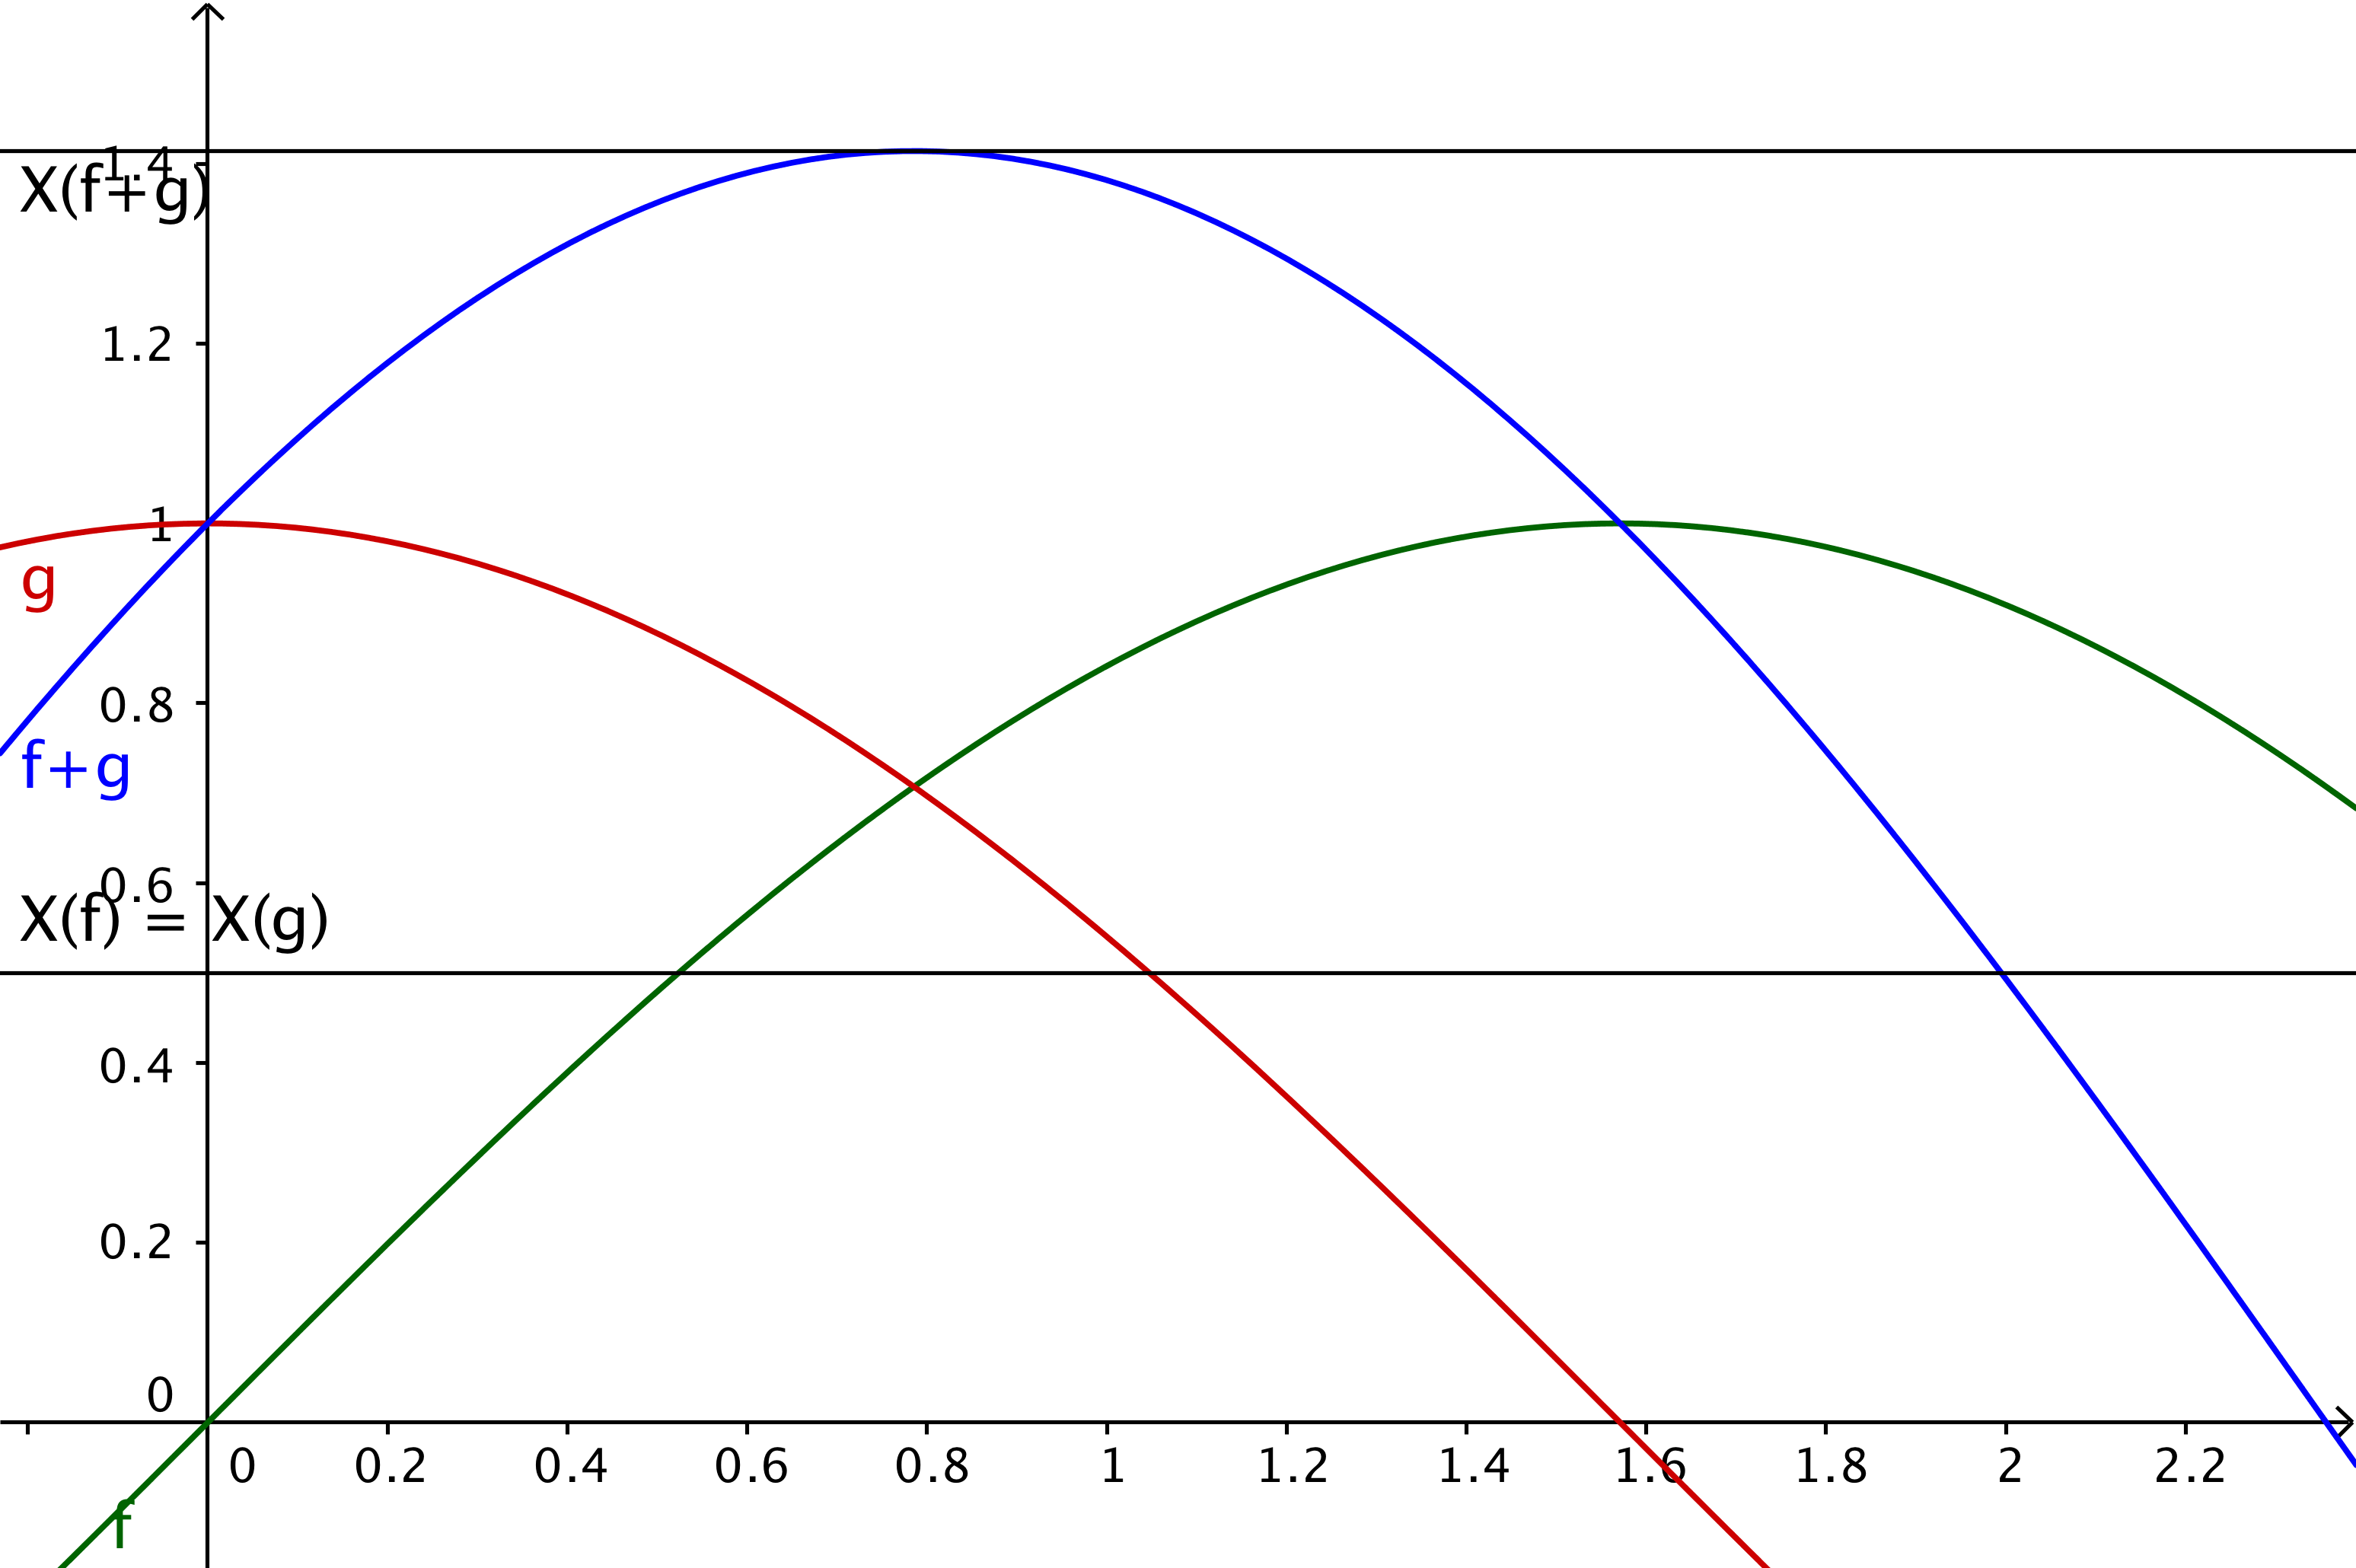
\includegraphics[scale = 0.5]{figtask6.png}
\caption{Plot of the functions and their best minimax approximations}
\label{figtask6}
\end{figure}
\qed
\end{document}

%%% Local Variables:
%%% mode: latex
%%% TeX-master: "report"
%%% End:



% \begin{problem}
  Let $\mathcal{A}$ be the 3-dimensional space of functions on
  $[-1,1]$ composed of two straight line segments joined at $x =
  0$. Calculate the element of $\mathcal{A}$ that minimizes
  \begin{equation}
    \label{eq:integral}
\int_{-1}^1 \lvert x^2 - p(x) \rvert \, \text{dx}, \quad p \in \mathcal{A}.
\end{equation}
\end{problem}


\begin{solution}
$\mathcal{A}$ is a Haar space as if a function in $\mathcal{A}$ has
more than 2 zeros it is identically zero. Which can be taken as the
definition of a Haar space.

We then note that equation \ref{eq:integral} is the 1-norm and the
element in $\mathcal{A}$ we are searching for is the best $L_1$
approximation from $\mathcal{A}$ to $x^2$. Now we use our dear theorem
14.5 again, giving us the zeros of the error function. These are given
by equation~\ref{eq:zeros}.
\begin{equation}
  \label{eq:zeros}
\zeta_k = \cos{\left (\pi \left(- \frac{k}{4} + \frac{3}{4}\right)
  \right )}
  \Leftrightarrow
  \begin{cases}
    \zeta_0 = - \frac{\sqrt{2}}{2} \\
    \zeta_1 = 0 \\
    \zeta_2 = \frac{\sqrt{2}}{2} \\
  \end{cases}
\end{equation}

By demanding that the error function have these three zeros we get a
candidate for a best approximation $p^*$ in
equation~\ref{eq:pstar}.

\begin{equation}
  \label{eq:pstar}
  p^*(x)  = 
  \begin{cases}
    - \frac{\sqrt{2} x}{2} & \text{for}\: x \in [-1, 0) \\
    \frac{\sqrt{2} x }{2} & \text{for}\: x \in [0, 1]    
  \end{cases}
\end{equation}

\begin{equation}
  \label{eq:task_4:error}
  x^2 - p^*(x)  = 
  \begin{cases}
    x^{2} + \frac{\sqrt{2} x}{2} & \text{for}\: x \in [-1, 0) \\
    x^{2} - \frac{\sqrt{2} x}{2} & \text{for}\: x \in [0, 1]
  \end{cases}
\end{equation}

The only thing remaining is to check that the criteria, from 14.4, of
there being exactly 3 zeros in the error function is meet. In this
case solving for all the zeros becomes solving a piece wise defined
second order polynomial which is indeed possible. One need not however
solve the equations explicitly. Instead we note that second order
polynomials can have at most 2 zeros and both parts of the error in
equation~\ref{eq:task_4:error} are second order polynomials with one
root in common ($x = 0$). We thus conclude that the error function has
at most 3 zeros and we know by construction that it has 3
zeros. Therefore we know it has {\bf exactly } three zeros. Thus we
have found an element of $\mathcal{A}$ that minimizes
equation~\ref{eq:integral}. Further as $\mathcal{A}$ is a Haar space
the best approximation is unique.

    
% \begin{figure}[!ht]
%   \centering
%   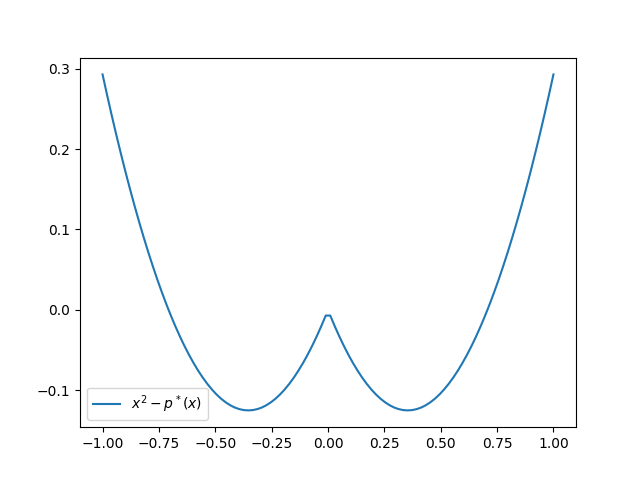
\includegraphics[scale = 0.5]{task_4_error.png}
%   \caption{Plot of $f - p^*$. Note that there is exactly 3 zeros!.}
%   \label{fig:task_3:error}
% \end{figure}

\end{solution}


%%% Local Variables:
%%% mode: latex
%%% TeX-master: "report"
%%% End:


% \begin{problem}
Let p be the cubic polynomial that interpolates the function values
$f(0)$, $f(1)$, $f(2)$, and $f(3)$. Express $p(6)$ in terms of $f(0)$,
$f(1)$, $f(2)$, $f(3)$, and verify that your formula is correct when
$f$ is the function ${f (x) = (x − 3) 3 ; 0 ≤ x ≤ 6}$ What is the
uncertainty in the value of $p(6)$, if the uncertainty in each function
value is $\pm \epsilon$?
\end{problem}

%--------------------------------------------------------------------%

\begin{solution}  

\end{solution}

%%% Local Variables:
%%% TeX-master: "report.tex"
%%% End:


% \begin{problem}
Show that the Chebyshev polynomials are mutually orthogonal relative to the
weight $w(x) = (1 − x 2 )^{−1/2}$ on $[−1, 1]$, that is
\begin{equation*}
  \int_{-1}^1 \frac{T_n(x) T_m(x)}{\sqrt{ 1- x^2}} dx = 0
\end{equation*}
\end{problem}

%--------------------------------------------------------------------%

\begin{solution}  

\end{solution}

%%% Local Variables:
%%% TeX-master: "report.tex"
%%% End:


\end{document}

%%% Local Variables:
%%% mode: latex
%%% TeX-master: t
%%% End:
